\section{Objectives}

Compare static, dynamic, and weak-feedback DFFs following handout PDF pages 74--77, covering hazards, noise immunity, frequency limits, and asynchronous reset. The circuits use transistors and TGs rather than ideal edge-triggered behavioral models.

\section{Handout requirements and test mapping}

\begin{center}
\small
\setlength{\tabcolsep}{4pt}
\begin{tabular}{p{.42\linewidth}p{.29\linewidth}p{.18\linewidth}}
\toprule
Requirement & Deck prefix and conditions & Status \\
\midrule
Step 1: hazards, latch versus DFF & 01; 20 ns period & Waveforms measured \\
Step 1: operating-frequency limit & 03; 12 periods & Finite boundary located \\
Step 2: equal-noise comparison & 02; 1/5/20 fF & Measured \\
Fig. 17.1(c): weak feedback & 01/02 & Compared \\
Q1--3: overlap, slope, setup/hold & Theory; Lab21 sweep & Analyzed; not full extraction \\
Q4: reset-low DFF & 04; both phases & Measured \\
\bottomrule
\end{tabular}
\end{center}

\section{Circuit and timing derivation}

Two TG latches use complementary clocks: the master is transparent during low phase and the slave during high phase, producing a positive-edge capture path. The static circuit uses switched feedback at both storage nodes. The dynamic circuit removes feedback and stores charge parasitically. The weak-feedback circuit uses long-channel weak inverters. Feedback loading, restoration current, and contention with new data jointly affect speed.

Asynchronous reset replaces the slave output inverter with a NOR: $Q=\overline{Z+R}$, forcing low when $R=1$. This verifies output reset, not a complete reset recovery/removal timing signoff.

\section{Simulation setup and interpretation}

The supplied encrypted MOS model is evaluated at a baseline supply of 1.0 V and 25\,$^\circ$C. The 1.0 V value is a teaching condition, not a verified voltage rating. These results do not reproduce the handout's original process or supply conditions. Unless stated in the deck, $W_n/W_p/L=0.6/1.8/0.25\,\mu\mathrm m$, bulks are tied to their corresponding rails, and output load is 5 fF. Transmission-gate and weak-feedback dimensions are specified explicitly in each deck.

PrimeSim HSPICE S-2021.09 win64 was used with \texttt{RUNLVL=6}, \texttt{ACCURATE}, and \texttt{WARNLIMIT=100}. Every baseline and \texttt{.alter} analysis concluded without errors or failed measurements. The simulator still reports suppressed warnings associated with encrypted blocks; this does not establish that the model is warning-free or that those warnings are harmless. The \texttt{.tran} print interval is not a fixed integration step: the solver uses adaptive timesteps. A finite sweep is not a complete process qualification.

Unless stated otherwise, the declared functional diagnostic uses $V\leq0.2$ V for low and $V\geq0.8$ V for high. These are report-level interpretation thresholds, not numerical handout requirements or extracted receiver noise margins. Correct samples do not exclude glitches between samples. Figures are redrawn from actual simulation data; \texttt{results/} contains per-case waveforms, measurements, and derived comparison CSV files.

Public decks omit model loading paths; model configuration is added only to local execution copies. The model itself is not distributed. The first two filename digits identify the deck numbers used below. Every deck is standalone.

\section{Results}

\begin{figure}[htbp]
\centering
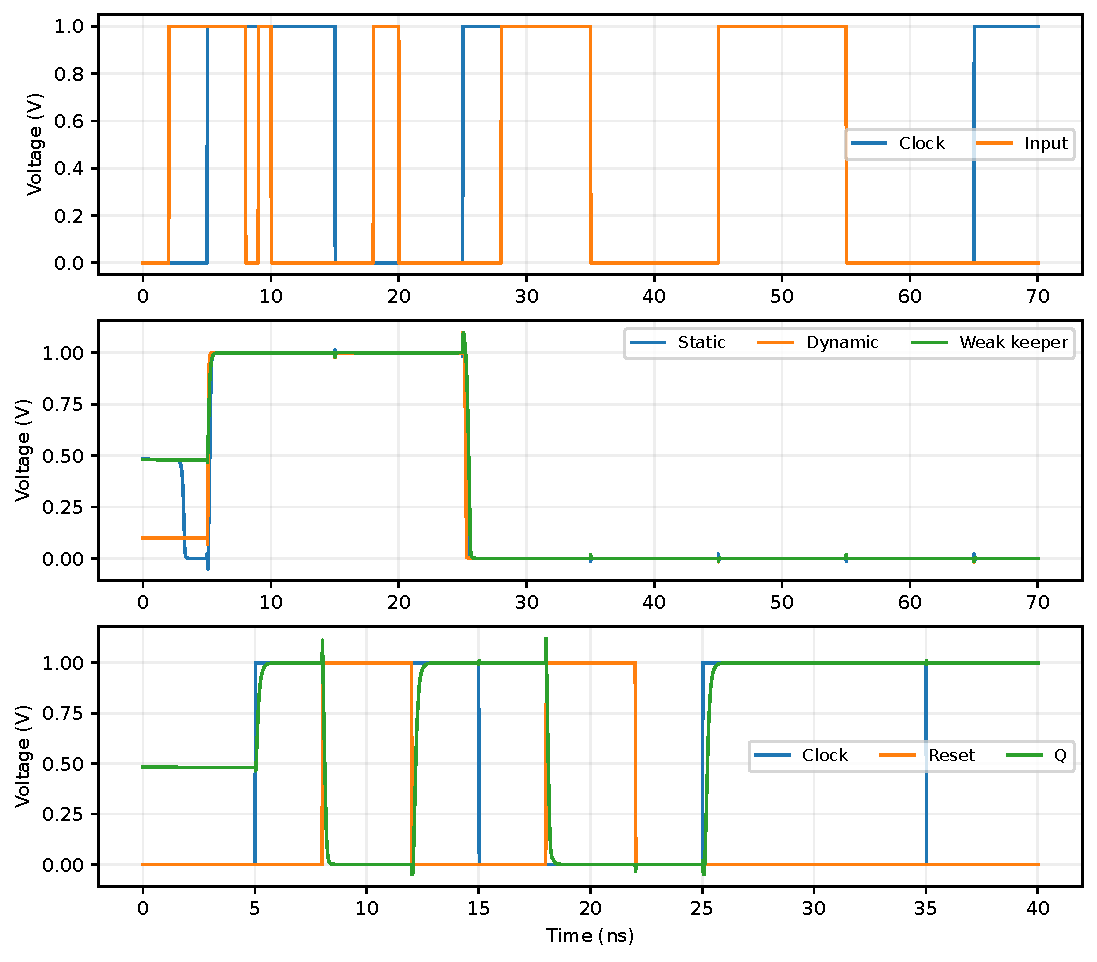
\includegraphics[width=.96\linewidth]{figures/hazards_and_reset.pdf}
\caption{The upper plots show data hazards and the three DFF outputs; the lower plot shows asynchronous reset in both clock phases.}
\end{figure}

The three circuits produce approximately 1, 0, 0, and 0 V at 7, 27, 47, and 67 ns. Pulses during the closed phase do not directly propagate to the output. The 45 ns data transition deliberately lies near the sampling edge and the setup/hold boundary; one waveform cannot prove that all near-edge hazards are safely rejected.

\begin{center}
\small
\setlength{\tabcolsep}{4pt}
\begin{tabular}{lrrr}
\toprule
Coupling (fF) & Static peak (V) & Dynamic peak (V) & Weak-feedback peak (V) \\
\midrule
1 & 0.00263 & 0.01208 & 0.01641 \\
5 & 0.00375 & 0.00814 & 0.01172 \\
20 & 0.06041 & 1.04148 & 0.99972 \\
\bottomrule
\end{tabular}
\end{center}

\begin{figure}[htbp]
\centering
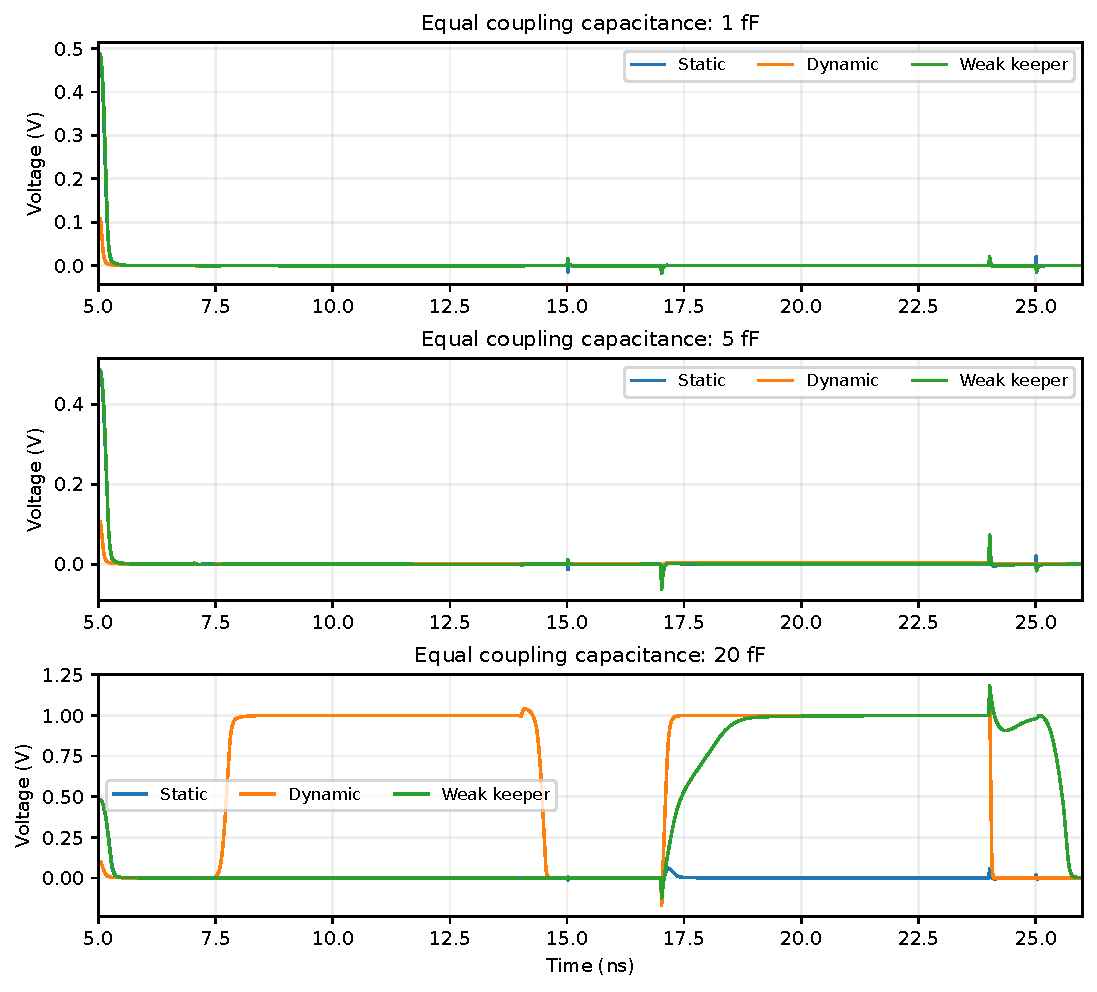
\includegraphics[width=.96\linewidth]{figures/noise.pdf}
\caption{Identical capacitors and aggressors couple into the master/slave storage nodes with input fixed at 0.}
\end{figure}

Under the strong 20 fF disturbance, the static output peaks at only 0.06041 V, while dynamic and weak-feedback outputs reach approximately 1.04148 and 0.99972 V, producing erroneous highs. Weak feedback does not reject arbitrarily strong disturbances. The small 1/5 fF peaks need not be monotonic because the measurement includes different injection phases and restoration dynamics.

\subsection{Frequency boundary and reset}

\begin{center}
\small
\setlength{\tabcolsep}{4pt}
\begin{tabular}{lrrr}
\toprule
Period (ns) & Frequency (GHz) & Static correct/8 & Dynamic correct/8 \\
\midrule
2 & 0.5000 & 8 & 8 \\
1.8 & 0.5556 & 8 & 8 \\
1.6 & 0.6250 & 8 & 8 \\
1.4 & 0.7143 & 4 & 8 \\
1.2 & 0.8333 & 4 & 8 \\
1 & 1.0000 & 0 & 4 \\
\bottomrule
\end{tabular}
\end{center}

\begin{figure}[htbp]
\centering
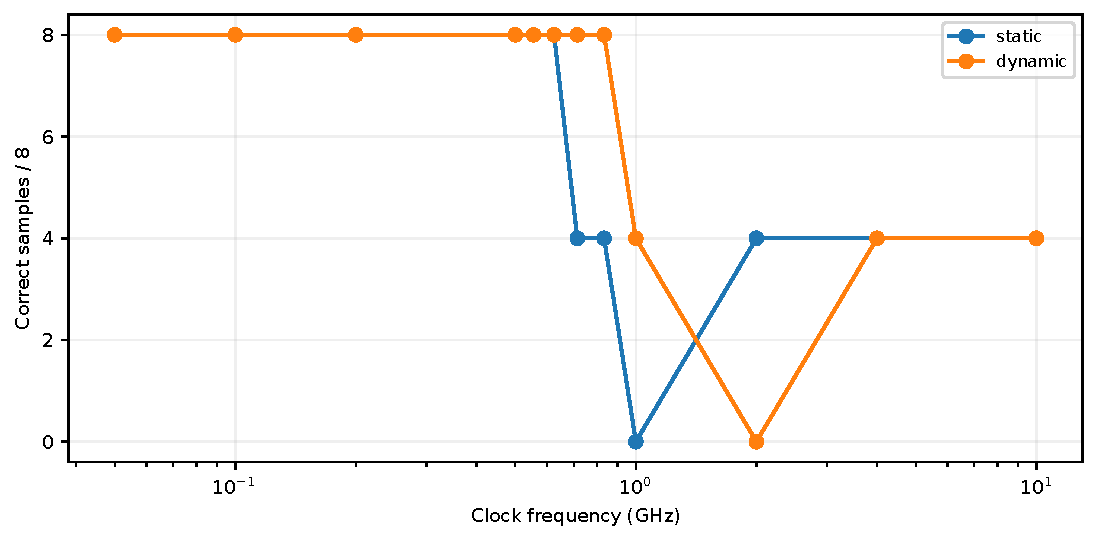
\includegraphics[width=.96\linewidth]{figures/frequency.pdf}
\caption{Fixed-time interpretation for 12 tested periods; connecting lines guide the eye and do not verify continuous frequencies.}
\end{figure}

The clock begins rising at $0.25T$ and outputs are sampled at $0.49T$, allowing about $0.24T$ to settle. The highest tested frequencies with 8/8 correct samples are 0.625 GHz (1.6 ns) for static and 0.8333 GHz (1.2 ns) for dynamic. Adjacent failing points are 0.7143 GHz (1.4 ns) and 1 GHz, respectively. These are finite-sweep boundaries under the stated load, 20 ps clock edge, and observation deadline, not unconditional $f_{\max}$ values.

Output during reset in high and low clock phases is 0.0001976 V and $3.395\,\mu$V, respectively; recapture after release gives 0.999979 V.

\section{Discussion, differences, and unverified scope}

Q1: overlapping conduction of complementary clocks can make master and slave transparent simultaneously and allow race-through. Q2: slow edges lengthen partial conduction and contention and alter available settling time, so nominal period alone is insufficient. Q3: setup allows the master storage node to settle before closing; hold prevents new data from crossing before closure completes. Both depend on clock slope, TG delay, and regeneration, rather than zero-time ideal logic. Continuous setup/hold and metastability extraction is not claimed; Lab21 separately measures slew and skew. Equal output loads and equal injected disturbances are used to avoid attributing mismatched tests to noise immunity.
